\chapter{Diskussion}

Im Folgenden werden die zuvor präsentierten Ergebnisse diskutiert. Zunächst werden die beobachteten Phänomene 
bei der Straßenerkennung betrachtet und daraufhin die bei der Radwegerkennung.

\section{Straßenerkennung}

Die Ergebnisse der Straßenerkennung können als gut im Vergleich zur Literatur eingeordnet werden. 
Das beste Modell ist hierbei das \ac{VBUNet}, welches mit einer Test-IoU von 64,26\% mit den 
performantesten Modellen aus \autoref{sec:state-of-the-art-roads} mithalten kann. Hier wurden 
Spitzenwerte von 67,10 und 65,60\% auf dem Massachusetts- bzw. Deep-Globe-Datensatz erzielt. 
Die Hyperparameter dieser Modelle sind auf das jeweilige Problem optimiert, während das VBUNet nicht optimiert ist. 
Dafür sind die Ergebnisse sehr gut. \\  
Was überraschend ist, ist, dass im Pre-Training in dieser Arbeit 
das VBUNet die besten Ergebnisse erzielt, während in der Literatur die besten Modelle ResNet-Derivate sind. 
Das kann daran liegen, dass in der Literatur die Modelle isoliert auf dem Massachusetts- und Deep-Globe-Datensatz 
trainiert werden. In dieser Arbeit sind alle Netze hingegen auf der Vereinigung der beiden Datensätze trainiert. 
Die beiden Datensätze stellen allerdings sehr unterschiedliche Landschaften dar. 
Möglicherweise funktioniert also ResNet, welches eine viel höhere Komplexität als VGG aufweist, besser 
als Spezialisierung auf einer der beiden Landschaften, ist also besonders angepasst auf die jeweilige Landschaft, 
während VGG mit der geringeren Komplexität besser Straßen generalisieren kann und deshalb robuster ist. 
Eine weitere, simplere Erklärung ist, dass in dieser Arbeit die Netze lediglich mit einem Satz 
an Hyperparametern und einem festen Seed genau ein mal trainiert sind. Außerdem sind die Ergebnisse 
nicht mit einer Kreuzvalidierung überprüft.
Es kann also lediglich eine schlechte Besetzung der Hyperparameter und Startwerte für das ResNet und eine 
gute für VGG vorliegen. \\
Der Erwartung entsprechend kann BUNet2 mit der eher geringen Parameteranzahl von 2 Mio. Parametern nicht 
mit der Leistung der restlichen Netze konkurrieren. BUNet15 zeigt, dass BUNet2 schlicht eine zu geringe 
Komplexität aufweist, um die Straßen so gut wie die komplexeren Netze segmentieren zu können. 
Trotzdem ist die Leistung nicht schlecht. Mit nur einem Bruchteil der Parameter der übrigen Netze
kann BUNet2 zumindest vergleichbare Ergebnisse erzeugen. \\
Während BUNet15 und BUNet2 bis auf die Parameteranzahl identisch sind, weswegen sich ein Unterschied in der 
Performance auf den Komplexitätsunterschied zurückführen lässt, ist bei dem Performance-Unterschied 
zwischen BUNet15 und den Backbone-Architekturen, insbesondere RBUNet und DBUNet, unklar, ob die kleine 
Differenz von wenigen Prozenten in der IoU bzw. der BIoU in der unterschiedlichen Architektur oder dem 
Pre-Training der Backbone-Architekturen auf ImageNet begründet ist. Eventuell ist RBUNet z.B. die schlechtere 
Architektur, erzielt aber bessere Ergebnisse als BUNet15 aufgrund des Pre-Trainings auf ImageNet. 
Ob das der Fall ist, kann nur durch weitere Experimente geklärt werden, die BUNet15 mit den nicht vortrainierten 
Backbone-Netzen vergleicht. In jedem Fall scheint aber das Pre-Training auf ImageNet nur geringe 
Performance-Verbesserungen herbeizuführen. 

\subsection{BIoU für die Straßenerkennung}

\begin{wrapfigure}{r}{0.40\textwidth}
	\centering
	\vspace{-20pt} % Manchmal möchte man den oberen Abstand selbst anpassen
	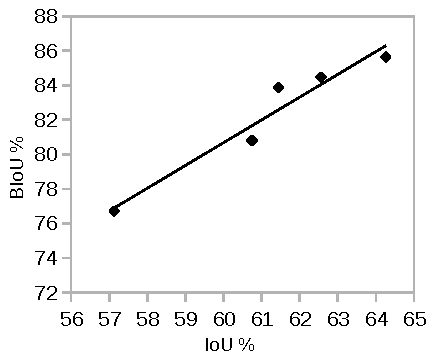
\includegraphics[width=0.35\textwidth]{Bilder/iou-biou-correlation.pdf}
	\vspace{-5pt}
	% Das folgende ist ein Trick, um "Abbilgung x.y" in eine
	% eigene Zeile zu packen. Der Text zwischen [ und ] steht
	% im Abbildungsverzeichnis. Der Text darunter wird
	% tatsächlich angezeigt.
	\caption[BIoU der Modelle der Straßenerkennung aufgetragen über deren IoU.]{\unskip}
	BIoU über IoU in Prozent (Straßenerkennung). Pos. Korrelation mit $r = 0,9707$. 
	\label{fig:iou-biou-corr}
	% \vspace{-20pt}
\end{wrapfigure}

Im Gegensatz zu den Radweg-Datensätzen bei der Maskenerstellung des Straßendatensatzes keinerlei Schätzung 
über die Lage der Wege eingesetzt worden. Die Masken sind also überwiegend deckungsgleich mit den tatsächlichen 
Straßen im Input-Bild, während bei den Radwegen manche Radwege grob versetzt positioniert sind. 
Deswegen muss die BIoU bei der Straßenerkennung keine komplette Verschiebung der Prediction zur Ground-Truth ausgleichen, 
sondern glättet lediglich die IoU im Randbereich der Straßen. Daher ist die Straßenerkennung geeignet, 
um zu untersuchen, ob die BIoU erwartungsgemäß arbeitet. \autoref{fig:iou-biou-corr} zeigt die Testergebnisse der 
Straßenerkennung mit der BIoU in Prozent aufgetragen über der IoU in Prozent für die jeweiligen Modelle. 
Es herrscht eine starke positive Korrelation zwischen der IoU und BIoU mit Korrelationskoeffizient $r = 0,9707$. 
Die starke Korrelation spricht für die vorangegangene Annahme, dass im Falle der Straßendetektion die BIoU 
ungerade Predictions glättet und fairer bewertet, bzw. näher an dem ist, wie ein Mensch die Performanz der 
Netze wahrnimmt. Die sehr streng bewertende IoU gibt einen schlechten Eindruck von der Leistungsfähigkeit des Netzes. 
Aus den Beispielpredictions der Straßenerkennung erhält ein menschlicher Beobachter nicht den Eindruck, 
dass nur circa 60\% der Straßen richtig erkannt worden sind, sondern eher im Bereich von 80\% oder mehr. 
Damit beweist sich die BIoU, als ein Maß, welches im Falle der Straßenerkennung lediglich die IoU so anhebt, 
dass eine zu schmal oder zu breit gezeichnete Predicition mit rauen Kanten als (qualitativ) korrekt in 
die Bewertung einfließt.  

\section{Radwegerkennung}

Die Ergebnisse für die Radwegerkennung (vgl. \autoref{tab:results}) zeigen, dass die Ergebnisse der 
Radwegerkennung statistisch signifikant\footnote{
	$p = 1,887\cdot 10^{-8}$ für IoU und $p = 3,77\cdot 10^{-7}$ für BIoU
	des einseitigen Zweistichproben-Welch-Test zwischen der Straßenerkennung 
	und der Radwegerkennung für Basic-Aug. 
} schlechter sind, als die der Straßenerkennung. Hierfür gibt es folgende Gründe:
\begin{enumerate}
	\item Das Problem der Radwegerkennung ist schwerer. Für die Radwegerkennung fällt es selbst Menschen schwer 
	diese auf Satellitenbildern zu erkennen. Für Fahrradstreifen am Straßenrand ist das noch gut möglich, 
	aber für oft überdeckte und überschattete Fahrradwege neben der Straße, die zum Beispiel durch einen Grünstreifen 
	von der Straße getrennt sind und mit dem Fußweg verbunden sind, ist schwierig festzustellen, ob ein Radweg 
	vorhanden ist, oder ob es sich nur um einen Gehweg handelt. Außerdem weisen Radwege weitaus 
	heterogenere Beläge auf, als städtische Straßen. Für Radwege kommen Asphalt, unterschiedlich farbene Pflastersteine,
	Schotter, rot oder grün gefärbter Asphalt und andere Untergründe zum Einsatz, 
	während die allermeisten Straßen in der Stadt aus Asphalt bestehen.
	Weiterhin gibt es viel weniger Radwege als Straßen, wodurch in den Trainingsdaten eine große Imabalance 
	und generell weniger Beispiele vorhanden sind, als in einem ähnlich großen Datensatz für die Straßenerkennung. 
	Auch unterscheiden sich Radwege zwischen Ländern und selbst Städten eines Landes weitaus stärker, als Straßen.
	\item Die automatisch generierten Annotationen sind überwiegend (ca. zu 83\%; vgl. \autoref{sec:quality-of-masks})
	auf dem Niveau einer Annotation durch Menschen, allerdings könnte der Anteil der Annotationen, die schlichtweg
	falsch sind, die Ergebnisse stark beeinträchtigen. Um diese Hypothese zu verifizieren sind weitere 
	Experimente mit einem besser annotierten Datensatz notwendig. Ein durch Menschen annotierter Datensatz 
	muss dafür klar definieren, was die Labelnden als Radweg anerkennen, da bei Radwegen auf Luftbildern 
	nicht unbedingt ein allgemeiner Konsens besteht, was als Radweg zu markieren zählt. Durch menschliche Annotation 
	kann aber zumindest ausgeschlossen werden, dass Pixel als Radweg annotiert sind, die eine Wiese oder ein Gebäude zeigen.
	\item Möglicherweise ist die semantische Segmentierung zum Erkennen der Radwege eine zu detaillierte Methode. 
	Um die Forschungsfrage dieser Arbeit -- existiert ein Radweg an dieser Straße und wenn ja, in welche Richtung -- 
	zu beantworten, ist die semantische Segmentierung der Radwege übermäßig. Die semantische Segmentierung 
	schafft mehr Informationen, als benötigt werden. Das bietet zwar auch Vorteile, dass zum Beispiel der Radweg 
	auf einem Luftbild als solcher eingefärbt werden kann, aber verlangt auch weitaus genauere Annotationen. \\
	Eine Alternative Herangehensweise kann sein, das Problem so zu modellieren, dass die Modelle direkt einen Graphen
	an Radwegen extrahieren, anstatt zuerst die zum Radweg gehörigen Pixel zu annotieren und die Graphenextraktion 
	in einem externen Schritt vorzunehmen. Dabei können als Label direkt die Graphen aus \ac{OSM} verwendet werden 
	und die Rad\textit{streifen} müssen nicht verschoben werden. Das Problem hierbei ist, zu Kodieren, ob 
	ein Radweg rechtsseitig oder linksseitig vorliegt, da die Definition von rechts- und linksseitig abhängt  
	von dem von \ac{OSM} willkürlich gewählten Verlauf der Straße. Hierfür könnte der Begriff von links- und 
	rechtsseitig transformiert werden in östlich und nördlich, bzw. in westlich und südlich von der Straße.    
\end{enumerate}
Obwohl die Radwegerkennung nicht so gute Ergebnisse liefert, wie die Straßenerkennung, und die Ergebnisse 
für die Radwegerkennung durchaus Verbesserungspotential bieten, lässt sich aus der Arbeit 
schließen, dass es möglich ist, andere Strukturen der städtischen Infrastruktur aus Luftbildern zu erkennen, 
als Straßen. 

\subsection{Ergebnisse auf Karlsruhe gegenüber BikeSat und Wolfsburg}

Aus allen Experimenten geht hervor, dass die Performance auf dem (ungefilterten und gefilterten) Karlsruhe-Datensatz deutlich schlechter ist, 
als auf dem BikeSat- und Wolfsburg-Datensatz. Außerdem hat die Color-Aug. keine Verbesserung gegenüber 
Basic-Aug. hervorgerufen. Auch ist der Wolfsburg-Datensatz, der eine andere Stadt, bei gleicher Optik der Bilder, 
zeigt, als der BikeSat-Datensatz, gleich auf mit dem BikeSat-Datensatz. Wolfsburg weist aber eine sehr ähnliche 
Infrastruktur zu den anderen Städten aus Niedersachsen (BikeSat) auf. Daraus lässt sich schließen, 
dass für die schlechte Performance auf dem Karlsruhe-Datensatz wahrscheinlich nicht die Optik der Bilder verantwortlich 
ist, sondern die sehr unterschiedliche Infrastruktur der Fahrradwege oder das allgemeine Stadtbild. 
So hat Karlsruhe beispielsweise deutlich mehr Fahrradstreifen am Straßenrand als die niedersächsischen Städte. 
Diese Beobachtung beantwortet die Forschungsfrage, ob Ergebnisse auf Städten unterschiedlicher Infrastrukturen 
übertragbar sind. So ist eine Übertragung bedingt möglich, aber es liegt nahe, dass mit Performance-Einbußen zu rechnen ist, 
die die Stärke des Unterschieds der Infrastrukturen widerspiegeln. 
Um diese These zu belegen, bedarf es jedoch weiterer Experimente mit mehr Städten. Eventuell ist dann 
auch eine Proportionalität zwischen Performance-Einbußen auf für das Modell unbekannten Städten und der Stärke 
des Unterschieds der Städte erkennbar. Insofern eine Quantifizierung des Unterschieds der Städte gelingt. 

Die signifikant bessere BIoU von Wolfsburg im Gegensatz zu BikeSat wird darauf zurückgeführt, dass 
Wolfsburg eine sehr ähnliche Fahrrad-Infrastruktur aufweist, wie der BikeSat-Datensatz, aber weniger 
Samples beinhaltet, die schwierig als Radweg zu erkennen sind. Außerdem ist der Unterschied nur gering, 
da der Unterschied in IoU keine statistische Signifikanz erreicht. 

% schlechtere Ergebnisse als Straßenkennung, was probleme ? 
% warum karslrueh so viel schlechterbiou
% warum wolfsburg besser ? 
% Wolfsburg doch eher ungeeignet weil zu ähnlich 
% experimente mit anderen städten
% color augmentation nicht viel grebracht -> liegt wohl an stadtbild
% netze eher konservativ wie karlsrueh prediction zeigt
% warum gefilterter schlechter?

effizienz des pretraining 
warum wenig unterschiede zwischen den netzen

\subsection{Effektivität des Fine-Tunings}



\subsection{BIoU für Radwegerkennung}

\subsection{Gefilterter Straßendatensatz}

\newcommand{\overbar}[1]{\mkern 8mu\overline{\mkern-8mu#1\mkern-8mu}\mkern 8mu}

Sei $K_{fil} \subset K_{unfil}$ mit $|K_{fil}| = 49; ~|K_{unfil}| = 196$ der gefilterte Kalrsruhe-Datensatz 
als Teilmenge vom ungefilterten Karlsruhe-Datensatz $K_{unfil}$. Wobei gefiltert bedeutet, dass 
keine leere Ground-Truth-Maske existiert, alle Bilder also einen Radweg enthalten.
Die Ergebnisse aus \autoref{tab:results} und \autoref{tab:results-ka-small} mit der Visualisierung aus 
\autoref{fig:iou-biou-corr-ka} zeigen, dass die BIoU auf dem gefilterten Datensatz $K_{fil}$ signifikant 
schlechter ist, als auf dem ungefilterten. Da die BIoU als aritmethisches Mittel der BIoU-Werte der einzelnen Bilder 
berechnet wird und die Predictions auf den Bildern von $K_{fil} \cap K_{unfil} = K_{fil}$ gleich ausfallen, 
lässt sich aus den durchschnittlichen Ergebnissen den beiden Datensätze die durchschnittliche BIoU auf den leeren Bildern 
$K_{leer} := K_{unfil} \setminus K_{fil};~ |K_{leer}| = |K_{unfil}| - |K_{fil}| = 147$ über   
\begin{align}
	\overbar{BIoU_{K_{unfil}}} = \frac{|K_{fil}| \cdot \overbar{BIoU_{K_{fil}}} + |K_{leer}| \cdot \overbar{BIoU_{K_{leer}}}}{|K_{unfil}|} \nonumber \\
	\label{eq:ka-empty}  \implies \overbar{BIoU_{K_{leer}}} = \frac{|K_{unfil}| \cdot \overbar{BIoU_{K_{unfil}}} - |K_{fil}| \cdot \overbar{BIoU_{K_{fil}}}}{|K_{leer}|} \\ 
	= \frac{196 \cdot \overbar{BIoU_{K_{unfil}}} - 49 \cdot \overbar{BIoU_{K_{fil}}}}{147} \nonumber
\end{align}
berechnen. Das ergibt \\ 
$\overbar{BIoU_{K_{leer}, basic}} = 56,36\%$ und \\ 
$\overbar{BIoU_{K_{leer}, color}} = 45,19\%$
für Basic-Aug. bzw. Color-Aug. Verglichen mit \\ 
$\overbar{BIoU_{K_{fil}, basic}} = 48,16\%; ~\overbar{BIoU_{K_{unfil}, basic}} = 23,58\%$ und \\
$\overbar{BIoU_{K_{fil}, color}} = 42,68\%; ~\overbar{BIoU_{K_{unfil}, color}} = 35,14\%$
sind die Werte also höher. Weiterhin gilt $\forall (x, y) \in K_{leer}: BIoU(Prediction_m(x), y) \in \{0; 1\}$ für alle Modelle $m$. 
Das liegt daran, dass die Ground-Truth $y$ per Definition von $K_{leer}$ stets leer ist, woraus folgt, dass die Kardinalität der 
Schnittmenge mit der Prediction für einen Input $x$ immer $0$ ist. Das heißt, die BIoU ist immer $0$, es sei denn 
das Modell $m$ annotiert keine Pixel als Radwege, dann ist die Kardinalität der Vereinigungsmenge auch $0$ und 
die BIoU per Definition gleich $1$. Selbige Schlussfolgerung gilt analog für die IoU. \\ 
Aus den Werten für $BIoU_{K_{leer}}$ folgt, dass in circa der Hälfte der Fälle die Modelle keinen einzigen Pixel 
(fälschlicherweise) als Radweg annotieren. Zusammen mit den Beispiel-Predictions aus \autoref{sec:example-preds} 
liegt die Vermutung sehr nahe, dass in der anderen Hälfte der Fälle nur sehr wenige Pixel von den Modellen 
fälschlicherweise als Radweg erkannt wurden. Daraus lässt sich eine sehr gute True-Negative-Rate und 
geringe False-Positive-Rate schließen, 
für deren Bewertung die ausgewählten Maßzahlen IoU und BIoU äußerst ungeeignet sind. Insofern lässt sich 
also ein gutes Ergebnis verzeichnen, dass die Modelle nicht jegliche Straßen mit Radwegen versehen und 
korrekt gelernt haben, was keine Radwege sind, obwohl die Modelle während des Trainings mit dem BikeSat-Datensatz 
nur Beispiele eingegeben bekommen haben, die Radwege enthalten. Es folgt, dass die Modelle eher hesitent sind,
Pixel als Radwege zu annotieren.  